\documentclass[11pt]{article}
\usepackage[margin=0.8in]{geometry}
\usepackage[T1]{fontenc}
\usepackage{lmodern,microtype,booktabs,graphicx,amsmath,xcolor,hyperref,xurl}
\hypersetup{colorlinks=true,urlcolor=blue,linkcolor=blue,pdftitle={When flight compression changes the query},pdfauthor={James N. Jean IV}}
\setlength{\parindent}{0pt}\setlength{\parskip}{6pt}\setlength{\tabcolsep}{5pt}
\newcommand{\ArchiveBytes}{37,509,701}
\newcommand{\NativeRows}{43,542}
\newcommand{\SourceScenes}{344}
\newcommand{\ChosenScenes}{24}
\newcommand{\WorkingPoints}{43,541}
\newcommand{\WorkingRuns}{106}
\newcommand{\SourceGaps}{28}
\newcommand{\DevAircraft}{13}
\newcommand{\FinalAircraft}{17}
\newcommand{\DevRuns}{41}
\newcommand{\FinalRuns}{65}
\newcommand{\DevChecks}{1,210,248}
\newcommand{\FinalChecks}{2,680,129}
\newcommand{\NativeChecks}{480,761}
\newcommand{\FixturePoints}{201}
\newcommand{\FixtureRetained}{2}
\newcommand{\FixtureBytes}{72}
\newcommand{\FixtureInputBytes}{6,440}
\newcommand{\EarlySeconds}{75}
\newcommand{\ReferenceExit}{126}
\newcommand{\ReplayExit}{51}
\newcommand{\AllBytes}{100.0}
\newcommand{\AllFails}{0}
\newcommand{\AllMax}{0.00}
\newcommand{\StrideTwoBytes}{50.2}
\newcommand{\StrideTwoFails}{52}
\newcommand{\StrideTwoMax}{640.08}
\newcommand{\StrideFourBytes}{25.3}
\newcommand{\StrideFourFails}{61}
\newcommand{\StrideFourMax}{640.08}
\newcommand{\StrideEightBytes}{12.8}
\newcommand{\StrideEightFails}{65}
\newcommand{\StrideEightMax}{640.16}
\newcommand{\StrideSixteenBytes}{6.6}
\newcommand{\StrideSixteenFails}{65}
\newcommand{\StrideSixteenMax}{649.94}
\newcommand{\GeoTenBytes}{16.5}
\newcommand{\GeoTenFails}{63}
\newcommand{\GeoTenMax}{701.52}
\newcommand{\GeoTwentyFiveBytes}{8.1}
\newcommand{\GeoTwentyFiveFails}{65}
\newcommand{\GeoTwentyFiveMax}{1038.37}
\newcommand{\GeoFiftyBytes}{4.3}
\newcommand{\GeoFiftyFails}{65}
\newcommand{\GeoFiftyMax}{1567.92}
\newcommand{\TimeTenBytes}{33.0}
\newcommand{\TimeTenFails}{12}
\newcommand{\TimeTenMax}{10.00}
\newcommand{\TimeTwentyFiveBytes}{14.1}
\newcommand{\TimeTwentyFiveFails}{14}
\newcommand{\TimeTwentyFiveMax}{25.00}
\newcommand{\TimeFiftyBytes}{5.7}
\newcommand{\TimeFiftyFails}{65}
\newcommand{\TimeFiftyMax}{49.94}
\newcommand{\AllMae}{0.00}
\newcommand{\AllMse}{0.00}
\newcommand{\AllRmse}{0.00}
\newcommand{\StrideEightMae}{10.30}
\newcommand{\StrideEightMse}{250.37}
\newcommand{\StrideEightRmse}{14.31}
\newcommand{\GeoTwentyFiveMae}{36.92}
\newcommand{\GeoTwentyFiveMse}{9761.50}
\newcommand{\GeoTwentyFiveRmse}{62.51}
\newcommand{\TimeTenMae}{1.89}
\newcommand{\TimeTenMse}{10.56}
\newcommand{\TimeTenRmse}{3.12}
\begin{document}
\begin{center}
{\LARGE\bfseries When flight compression changes the query}\par
\vspace{5pt}{\large An audit of point reduction, route length and zone timing}\par
James N. Jean IV \quad | \quad Independent research program, Study 40\par
October 30, 2026 \quad | \quad Not peer reviewed
\end{center}
\section*{The decision}
Smaller trajectory files help only when the questions asked of them still give acceptable answers. This study tests whether point reduction preserves position at the original sample times, horizontal route length, and time spent inside two circular zones. A visually similar route is not enough to establish that its timing survives replay.

\textbf{Finding.} Development used \DevRuns{} runs from \DevAircraft{} aircraft. Every point-reducing configuration failed at least one fixed fidelity budget on at least one run. The predeclared selection rule therefore retained all original point records. The final comparison, on \FinalRuns{} runs from \FinalAircraft{} different aircraft, preserved that decision without selecting another setting.

\textbf{Practical recommendation.} Keep the supplied records under these budgets. Before replacing them in a query system, test the actual downstream queries and calibrate their tolerances with domain users. The repository includes an offline implementation exercise that reports a failure or unavailable input instead of recommending an unchecked representation.

\textbf{What the byte comparison means.} Each encoded run has an 8-byte count followed by 32 bytes per retained point: elapsed time and three float64 coordinates. The comparison concerns this point-record representation, including its header. It does not measure compressed ZIP size, network cost, cloud savings or production speed.

\textbf{Authored acceptance budgets.} A run must keep maximum time-aligned position error at or below 25 m; absolute horizontal-route relative error at or below 1\%; and sampled occupancy and first-transition timing errors at or below 2 s for both 1 km and 2 km closed disks. Transition states must match. A configuration is eligible only if every development run passes every budget. These thresholds were fixed before source acquisition; they are not an operational safety standard.

\textbf{Important limits.} The reference is processed, cubic-interpolated 1 Hz data from one general-aviation airport. It is not sensor ground truth or a set of complete independent flights. This is a finite audit of standard reducers and supplied-record fidelity, not a claim that trajectory compression is universally ineffective. No airline-delay, deployment, safety or financial outcome was measured.

\clearpage
\section*{1. Source, cohort and chronological safeguards}
TrajAir documents aircraft trajectories around Pittsburgh--Butler Regional Airport (KBTP) from September 2020 to April 2021. Its official project page and Figshare record identify the dataset under CC BY 4.0. This audit uses the fixed \texttt{7days1.zip} file, Figshare file 28625121, associated with DOI \href{https://doi.org/10.1184/R1/14866251.v1}{the pinned dataset record}. The archive contains \ArchiveBytes{} bytes; its SHA-256 and publisher MD5 are recorded in the repository. Other weekly archives and weather members are outside the cohort.

The source plan selected the first \ChosenScenes{} numerically ordered processed scenes from \SourceScenes{} eligible scenes before coordinate values were acquired. The \NativeRows{} native rows form 79 scene/aircraft tracks. Twenty-eight gaps are present (\SourceGaps{} counted by the checker); they split runs instead of being bridged by additional interpolation. There are no duplicate-frame rows or out-of-order transitions. One one-point run fails the fixed 20-point minimum. The remaining \WorkingRuns{} runs contain \WorkingPoints{} points. The maximum permitted run length is 20,000 points.

Each source row supplies an integer frame, aircraft identifier, x/y/z positions in kilometres and two wind fields. Positions are converted to metres in a runway-centred Cartesian system; wind is not analysed. The source already applies filtering and cubic interpolation at 1 Hz. Elapsed integer times are measured separately within each retained contiguous run.

\textbf{Aircraft grouping.} SHA-256 of the literal prefix \texttt{trajair-aircraft-v1:} followed by the base-10 source aircraft identifier assigns even first bytes to development and odd first bytes to final evaluation. All appearances of an aircraft stay together across the chosen scenes. This produces \DevAircraft{} development aircraft and \FinalAircraft{} final aircraft, with \DevRuns{} and \FinalRuns{} runs respectively. The publisher's scene train/test labels are not the study split. Runs from one aircraft are dependent; a circuit may appear as more than one segment.

\textbf{What was and was not blinded.} All source coordinates were present for source-quality checks. Final compression and query scores were not calculated until the development selection and 34 analytical dependencies were committed and frozen. The protocol root is \texttt{e17b0aab0d3e}; the development checkpoint is \texttt{9163d28a59e8}; the dependency freeze is \texttt{324649f9bdbb}. Point-diagnostic evidence was added after the first development execution without changing its metric values, configurations or selection. The earlier evidence remains private.

\textbf{Publication boundary.} The public package contains aggregate metrics, ordinal run/group labels, retained indices and hashes, plus wholly authored example coordinates. Recorded trajectories, source aircraft identifiers, absolute source times and encoded coordinate payloads stay outside Git. Reproduction requires a separate download of the pinned public archive and then runs offline. Source rights do not imply that an operational use is validated.

\clearpage
\section*{2. Representations and the development decision}
The fixed grid contains identity; every 2nd, 4th, 8th or 16th point; geometric Douglas--Peucker at 10, 25 or 50 m; and a time-aware variant at those same tolerances. Endpoints and retained elapsed times are preserved. Geometric distance is measured to a finite three-dimensional chord, with its projection clamped to the segment. The time-aware residual compares each original point with the chord interpolated at that point's actual elapsed time. Zero-length chords, equal maximum residuals and exact tolerance equality have explicit fixture coverage. A split occurs only when the residual is strictly greater than the tolerance; the earliest maximum wins a tie.

For reference positions $p_i$ and decoded positions $\hat p_i$ at the original times, define $e_i=\|\hat p_i-p_i\|_2$. Per-run error summaries are
\[
 \mathrm{MAE}=n^{-1}\sum_i e_i,\qquad
 \mathrm{MSE}=n^{-1}\sum_i e_i^2,\qquad
 \mathrm{RMSE}=\sqrt{n^{-1}\sum_i e_i^2}.
\]
Component-wise signed bias is also retained. Horizontal route length sums two-dimensional consecutive segment lengths. When its reference length is zero, relative error is unavailable; the stationary case uses its explicitly defined absolute rule. Sampled zone occupancy counts interval starts and excludes the final point. First transition means the first sampled change of inside/outside membership. It is not a continuous boundary-crossing estimate; no, missed and false transitions remain distinct states.

\begin{center}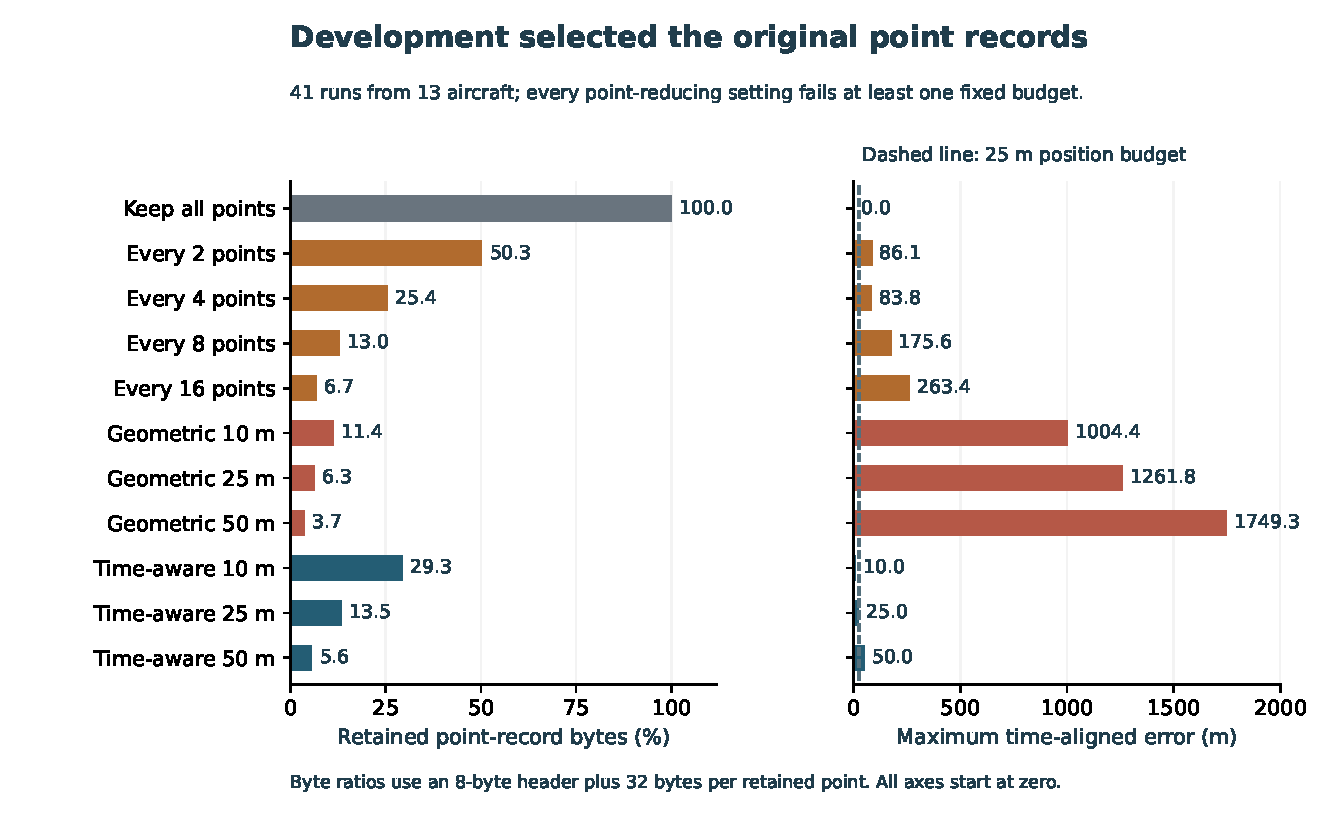
\includegraphics[width=\linewidth]{images/development_fidelity.pdf}\end{center}
\textbf{Selection.} Minimise summed encoded bytes among configurations passing every budget on every development run; break ties in the declared grid order. Only identity qualifies. The time-aware 10 m setting respects the position budget but fails route length on ten development runs. Geometric distance alone can preserve the route's shape while distorting its replay timing. No final score was used to alter the selector.

\clearpage
\section*{3. Final-aircraft comparison}
The selected identity representation passes all budgets and retains 100\% of the specified point-record bytes. The complete fixed grid is shown descriptively; there is no final-set reselection. Counts concern \FinalRuns{} runs, not independent flights.
\begin{center}\small
\begin{tabular}{lrrr}\toprule
Setting & Bytes retained (\%) & Failing runs & Max error (m)\\\midrule
Keep all points & \AllBytes{} & \AllFails{} & \AllMax{} \\
Every 2 points & \StrideTwoBytes{} & \StrideTwoFails{} & \StrideTwoMax{} \\
Every 4 points & \StrideFourBytes{} & \StrideFourFails{} & \StrideFourMax{} \\
Every 8 points & \StrideEightBytes{} & \StrideEightFails{} & \StrideEightMax{} \\
Every 16 points & \StrideSixteenBytes{} & \StrideSixteenFails{} & \StrideSixteenMax{} \\
Geometric 10 m & \GeoTenBytes{} & \GeoTenFails{} & \GeoTenMax{} \\
Geometric 25 m & \GeoTwentyFiveBytes{} & \GeoTwentyFiveFails{} & \GeoTwentyFiveMax{} \\
Geometric 50 m & \GeoFiftyBytes{} & \GeoFiftyFails{} & \GeoFiftyMax{} \\
Time-aware 10 m & \TimeTenBytes{} & \TimeTenFails{} & \TimeTenMax{} \\
Time-aware 25 m & \TimeTwentyFiveBytes{} & \TimeTwentyFiveFails{} & \TimeTwentyFiveMax{} \\
Time-aware 50 m & \TimeFiftyBytes{} & \TimeFiftyFails{} & \TimeFiftyMax{} \\
\bottomrule\end{tabular}
\end{center}
\begin{center}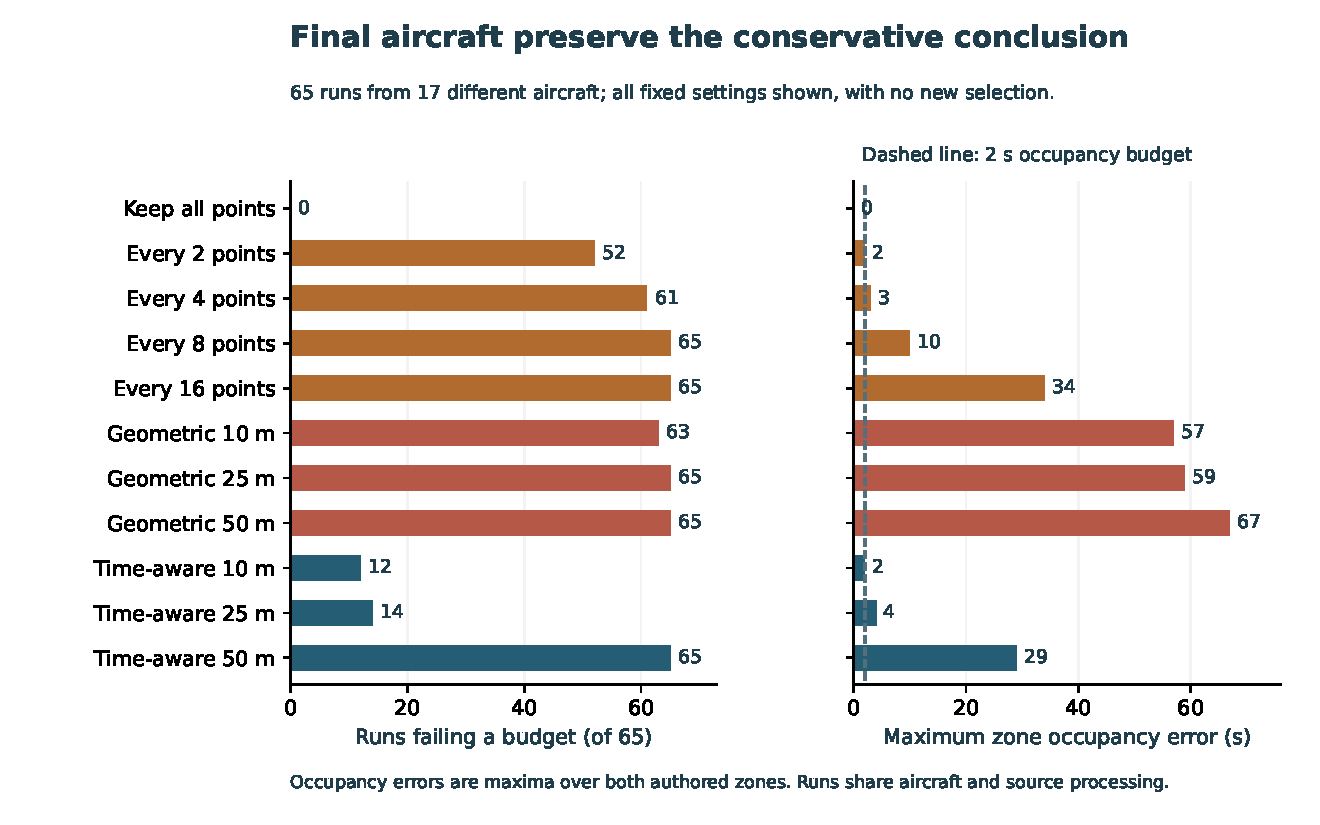
\includegraphics[width=0.94\linewidth]{images/final_query_failures.pdf}\end{center}
Time-aware 10 m fails only the route-length budget on twelve runs; its position and timing budgets pass. Geometric 25 m retains 8.1\% of point-record bytes but fails at least one budget on every final run. Its maximum time-aligned error exceeds one kilometre. These findings do not establish physically accurate motion: all error comparisons use the processed source reference.

\clearpage
\section*{4. Error scale and the implementation exercise}
The following values first average within each aircraft and then give every available aircraft equal weight. MAE and RMSE are in metres; MSE is in square metres. The macro RMSE is not the square root of macro MSE: averaging occurs after the per-run square root. Full bias, route, timing, availability denominators and run-level results remain machine-readable.
\begin{center}\small
\begin{tabular}{lrrr}\toprule
Setting & MAE (m) & MSE (m$^2$) & RMSE (m)\\\midrule
Keep all points & \AllMae{} & \AllMse{} & \AllRmse{} \\
Every 8 points & \StrideEightMae{} & \StrideEightMse{} & \StrideEightRmse{} \\
Geometric 25 m & \GeoTwentyFiveMae{} & \GeoTwentyFiveMse{} & \GeoTwentyFiveRmse{} \\
Time-aware 10 m & \TimeTenMae{} & \TimeTenMse{} & \TimeTenRmse{} \\
\bottomrule\end{tabular}
\end{center}
\textbf{Authored timing counterexample.} A 201-point teaching path stays at its initial location for 100 s, then moves along a straight line to 4,000 m at 200 s. Geometric simplification keeps \FixtureRetained{} of \FixturePoints{} points and encodes \FixtureBytes{} bytes instead of \FixtureInputBytes{}. The route length is exactly preserved, but time interpolation starts moving immediately. The first sampled exit from the closed 1 km disk changes from \ReferenceExit{} s to \ReplayExit{} s, which is \EarlySeconds{} s early. This is an authored mathematical example, not a recorded aircraft event or operational outcome.
\begin{center}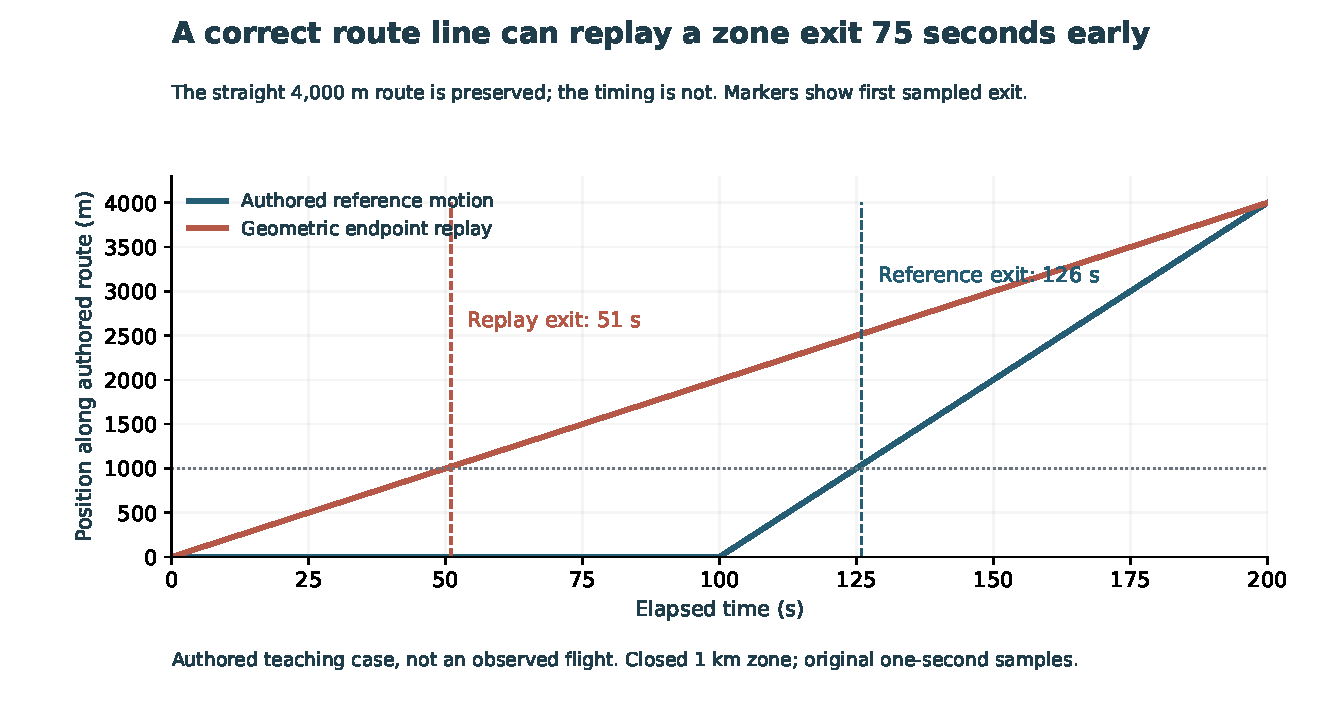
\includegraphics[width=\linewidth]{images/authored_timing.pdf}\end{center}
\textbf{Try the guard.} Run \texttt{python src/exercise.py --help} for the local CSV interface. The safe constant-speed example passes; the timing counterexample fails; and the incomplete-time example returns unavailable input with no metrics. The exercise checks supplied records under the authored budgets. It neither controls aircraft nor recommends an operational trajectory. Its three cases have 18 independent closed-form checks.

\clearpage
\section*{5. Verification, scope and next evidence}
A separate native-source checker reparses the ZIP and uses SQLite gap boundaries and 70-digit Decimal conversion checks: \NativeChecks{} conditions pass. The numerical checker imports none of the analysis helpers. It independently decodes the actual encoded records and per-point diagnostics, verifies the split trees and strict branch rules, reconstructs with 80-digit Decimal arithmetic, and recomputes group summaries and selection using SQLite. It passes \DevChecks{} development conditions and \FinalChecks{} final conditions. These are finite condition counts, not a universal correctness claim.

Complete full-history analysis replays at checkpoint \texttt{d3d630f4c9d2} pass on CPython 3.10.11 and 3.12.14, each using NumPy 2.2.5. Each replay checks 168,193 exact facts and 16,863 numeric facts under the predeclared tolerances, plus 2,340 regenerated runtime-specific hashes. All source-member identities, counts, states, retained indices and encoded payload bytes match exactly. Numeric tolerances are $10^{-8}$ m for point/error distances, $10^{-6}$ m$^2$ for MSE, $10^{-6}$ m for accumulated route lengths and $10^{-10}$ for ratios. Query times, guards and selection remain exact. As-run diagnostic hashes may differ across runtimes; their independently decoded facts must still pass. The source archive hash is unchanged. Thirty-four fixture methods also pass. Public figure verification checks plotted SVG geometry and numeric labels against checked results, rather than trusting the rendering call.

\textbf{Limits that affect interpretation.} This convenience cohort covers a small part of one public archive at one airport. Aircraft separation prevents identity overlap across study phases; it does not remove shared weather, airspace or source-processing dependence. The 1\% route-length budget could preserve source fluctuations as well as useful movement, and its operational appropriateness has not been calibrated. Large processed-reference errors are not evidence of true physical jumps. There is no counterfactual operational trial, latency benchmark, financial estimate or safety validation. The fixed grid is finite; failure here does not prove that every reducer or every less strict use case must fail.

\textbf{Next evidence.} Agree query tolerances with the intended users, inspect source fidelity through an approved independent reference, and freeze a new cohort and protocol before testing a revised representation. Preserve the present failures as evidence. Do not relax the current budgets or remove difficult runs to turn this audit into a positive result.

\textbf{Sources and attribution.}\par
\small
Patrikar, J., Moon, B., Ghosh, S., Oh, J., and Scherer, S. TrajAir: A General Aviation Trajectory Dataset (2021). \url{https://theairlab.org/trajair/}; dataset DOI \url{https://doi.org/10.1184/R1/14866251.v1}; research description \url{https://arxiv.org/abs/2109.15158}. Source data licensed CC BY 4.0. This study reports derived audit metrics and authored examples.\par
Douglas, D. H., and Peucker, T. K. Algorithms for the reduction of the number of points required to represent a digitized line or its caricature (1973). DOI \url{https://doi.org/10.3138/FM57-6770-U75U-7727}.\par
Meratnia, N., and de By, R. A. Spatiotemporal compression techniques for moving point objects (2004). DOI \url{https://doi.org/10.1007/978-3-540-24741-8_44}. Standard geometric and time-aligned ideas are used; no new compression algorithm is claimed.\par
Code, protocol, complete comparison and replay instructions: \url{https://github.com/S3R3Bii/flight-compression-query-audit}.
\end{document}
